\begin{titlepage}

	\centering

	\begin{tikzpicture}

		\node[opacity=0.3,inner sep=0pt,remember picture,overlay] at (4.5,-0.5){
\includegraphics[width= 0.95 \textwidth]{Figures/world.pdf}};

		\node[inner sep=0pt] (logo) at (0,0)
		{
\includegraphics[width=.20\textwidth]{Figures/flag.pdf}};

		\node[
			text width=0.5\textwidth,
			right=of logo,
			yshift=7.5,
			font=\sffamily\huge\linespread{1.0}\selectfont,
			execute at begin node=\setlength{\hyphenpenalty}{10000}\setlength{\exhyphenpenalty}{10000}
		] (title) {\reporttitle};

		\node[text width = 0.5\textwidth, yshift = 0.75cm, below = of title](subtitle){\sffamily\large \reportsubtitle};

		\node[text width = 0.5\textwidth, yshift = 0.90cm, below = of subtitle](version){\sffamily\large \reportversion};

		\gettikzxy{(subtitle.south)}{\sffamily\subtitlex}{\subtitley}
		\gettikzxy{(title.north)}{\titlex}{\titley}
		\gettikzxy{(logo.north)}{\logox}{\logoy}
		\pgfmathsetlengthmacro{\linetopy}{1.50 * \subtitley}
		\pgfmathsetlengthmacro{\linebottomy}{1.50 * \logoy}
		\draw[line width=.25mm, main-color]($(logo.east)!0.5!(title.west)$) +(0, \linetopy) -- +(0, \linebottomy);

	\end{tikzpicture}
	\vspace{3cm}

	\sffamily\groupnumber

	\begin{table}[H]
		\centering
		\sffamily
		\large
		\begin{tabu} to 0.8\linewidth {cc}
			\textbf{Családnév} & \textbf{Keresztnév} \\
			\hline

			\sffamily\reportauthors
		\end{tabu}

	\end{table}

	\tikz[remember picture,overlay]\node[anchor=south,inner sep=0pt] at (current page.south) {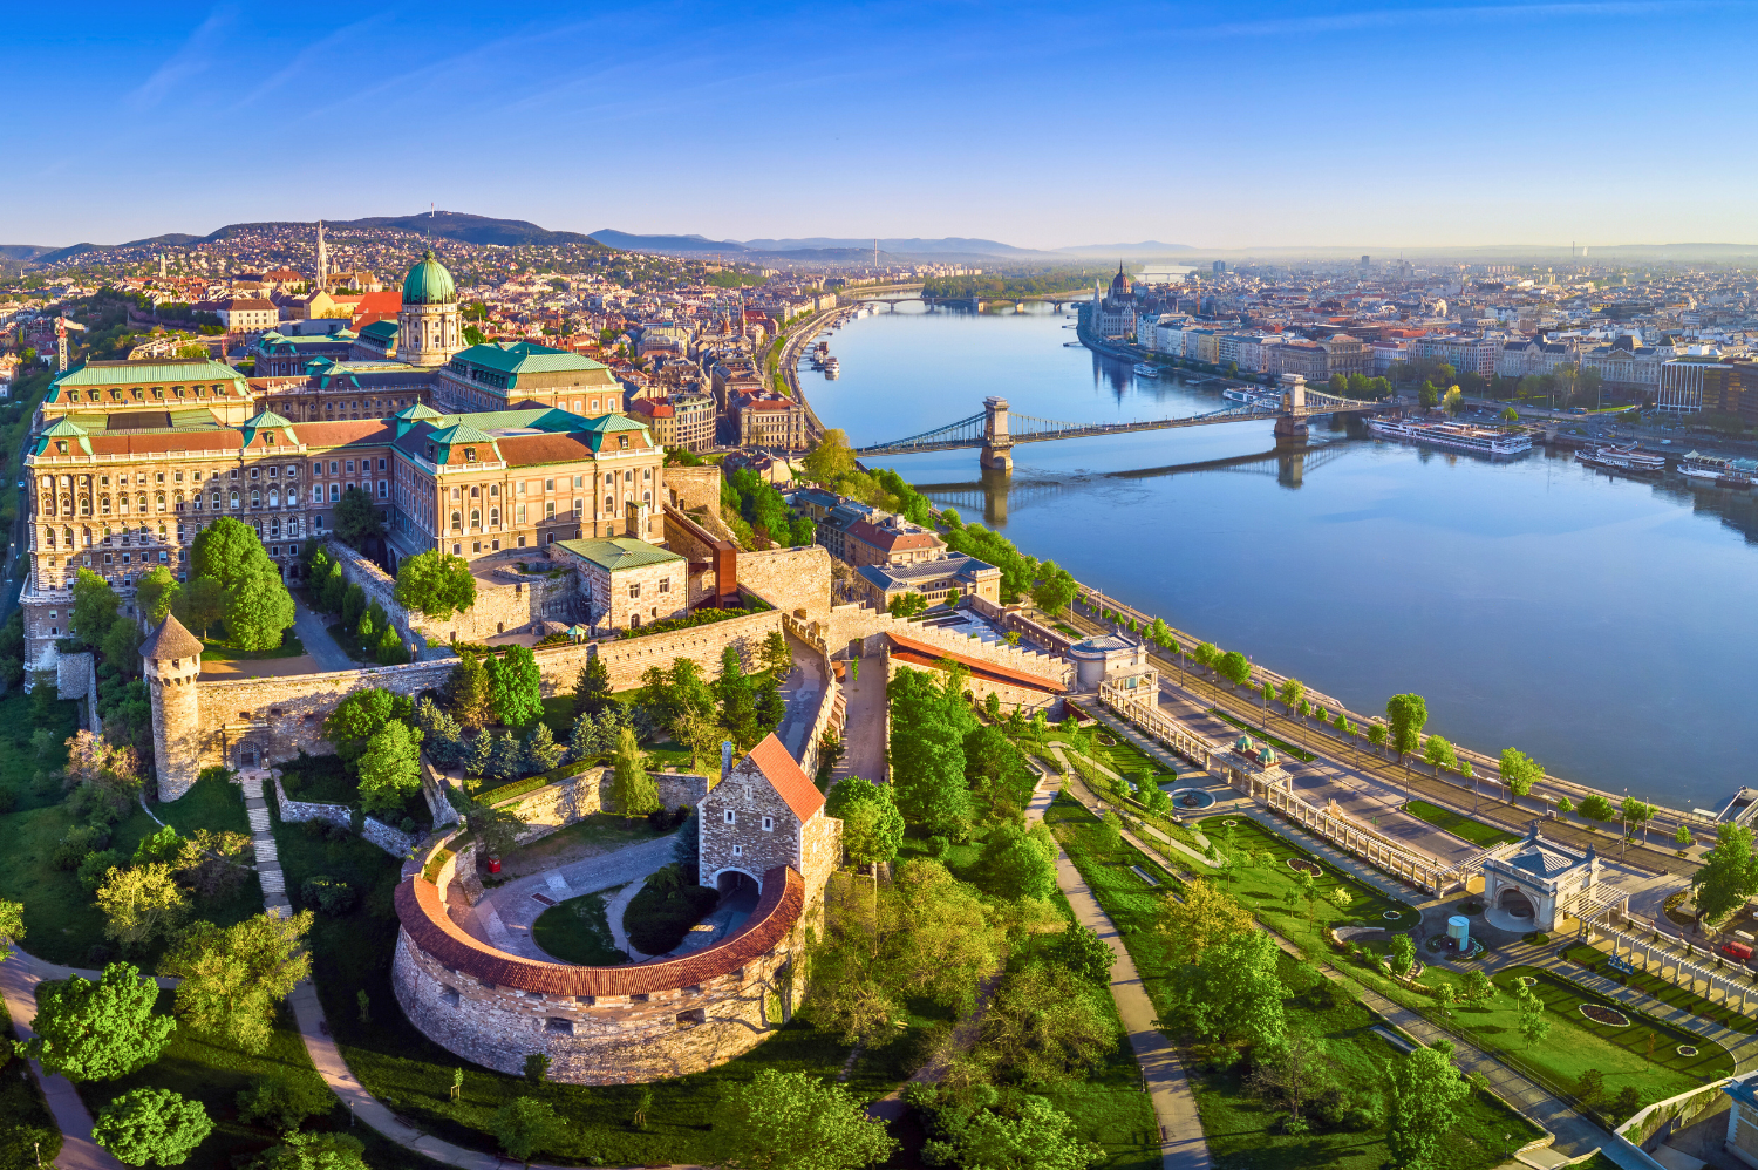
\includegraphics[width=\paperwidth]{Figures/landmark.pdf}};

\end{titlepage}








